\documentclass[letterpaper,twocolumn,10pt]{article}
\usepackage{usenix-2020-09}
\usepackage{booktabs}
\usepackage{graphicx}
\usepackage{xspace}
\usepackage{url}

\newcommand{\system}{LatchMoE\xspace}

\title{LatchMoE: Graph-Compatible Expert Offloading through Address-Stable Residency}

\author{Anonymous submission}

\begin{document}
\maketitle

\begin{abstract}
Sparse mixture-of-experts (MoE) models reduce arithmetic per token but retain a
large parameter footprint.  Expert offloading can fit such models on a
memory-constrained accelerator, yet conventional offloading changes weight
locations on the decode path.  This behavior conflicts with graph replay,
which relies on stable addresses and a repeatable execution topology; disabling
replay exposes a host-bound decode path.

We present \system, an expert-offloading runtime that separates dynamic expert
residency from captured tensor addresses.  \system preallocates fixed device
slots, stages routed experts outside the replay boundary, protects slots with
an explicit transfer/compute lifecycle, and executes oversized prefill working
sets in capacity-bounded waves.  The resulting data plane accepts placement
plans without embedding a particular prediction policy.

The implementation targets a hook-enabled vLLM-Ascend stack.  A graph-only
lifecycle qualification on Qwen3-30B-A3B records exact output agreement,
stable addresses, transfer ordering, bounded residency, and service release
across three independent starts.  Historical capture-disabled diagnostics are
excluded.  We treat the online result as narrow mechanism evidence and still
require matched graph-compatible baselines and a broader matrix before making
a general performance claim.
\end{abstract}

\section{Introduction}
\label{sec:intro}

Mixture-of-Experts (MoE) architectures have emerged as a prominent approach for scaling Large Language Models (LLMs) to hundreds of billions of parameters~\cite{shazeer2017outrageously,fedus2022switch, jiang2024mixtral,dai2024deepseekmoe}. 
By dynamically routing each token to only a sparse subset of experts, MoE models substantially increase model capacity while keeping per-token computation bounded~\cite{du2022glam,rajbhandari2022deepspeedmoe}. 
However, sparse activation reduces computation rather than model storage: although only a small number of experts are activated for each token, the runtime must still make the entire expert pool available for routing. 
As MoE models scale, the simultaneous residency of all expert weights in accelerator High-Bandwidth Memory (HBM) places significant strain on memory capacity.
To serve such models on memory-constrained accelerators, \textbf{expert offloading} has become an important strategy: the runtime keeps non-expert layers and a bounded subset of frequently used experts in local HBM, while fetching non-resident experts from host memory on demand~\cite{hwang2024pregated,xue2024moeinfinity,li2026commitmoe}. 

To make expert offloading practical, prior systems reduce its data-movement overhead through expert caching, routing-aware prediction and prefetching, and transfer--computation overlap~\cite{hwang2024pregated,kong2024swapmoe,cao2025moelightning,fang2025klotski,xue2024moeinfinity}. 
These techniques reduce the frequency of host-to-device transfers or hide part of their latency, substantially improving the efficiency of offloaded MoE inference. 
However, they do not eliminate the inherent execution dynamism introduced by expert offloading. 
Loading and replacing experts in a bounded HBM cache can change the mapping between logical experts and their physical weight locations across decoding steps. 
Thus, existing data-movement optimizations improve which experts are moved and when they are moved, but they do not eliminate runtime changes in logical-to-physical weight bindings. 

Such runtime changes can be naturally accommodated under eager execution, where the host resolves the current expert placement and dispatches the corresponding kernels at each decoding step. This flexibility, however, comes at a substantial performance cost. Autoregressive decoding repeatedly executes a largely recurring sequence of fine-grained accelerator kernels, and launching these kernels individually incurs repeated host-side scheduling, dispatch, and synchronization overhead. \textbf{Graph replay} mitigates this overhead by capturing the recurring execution sequence once and replaying it as a unit, thereby reducing host-induced gaps between kernel executions~\cite{kwon2020nimble,ye2025flashinfer}. 

As shown in Figure~\ref{fig:graph_breakdown}, graph replay reduces average decode latency by approximately 75\% across four workloads, from 133.7--137.4~ms/token under eager execution to 32.6--33.6~ms/token, while device execution time remains nearly unchanged. 
This result indicates that most of the improvement comes from eliminating host-induced device idle time rather than accelerating the underlying kernels. 

\begin{figure}[t] 
  \centering 
  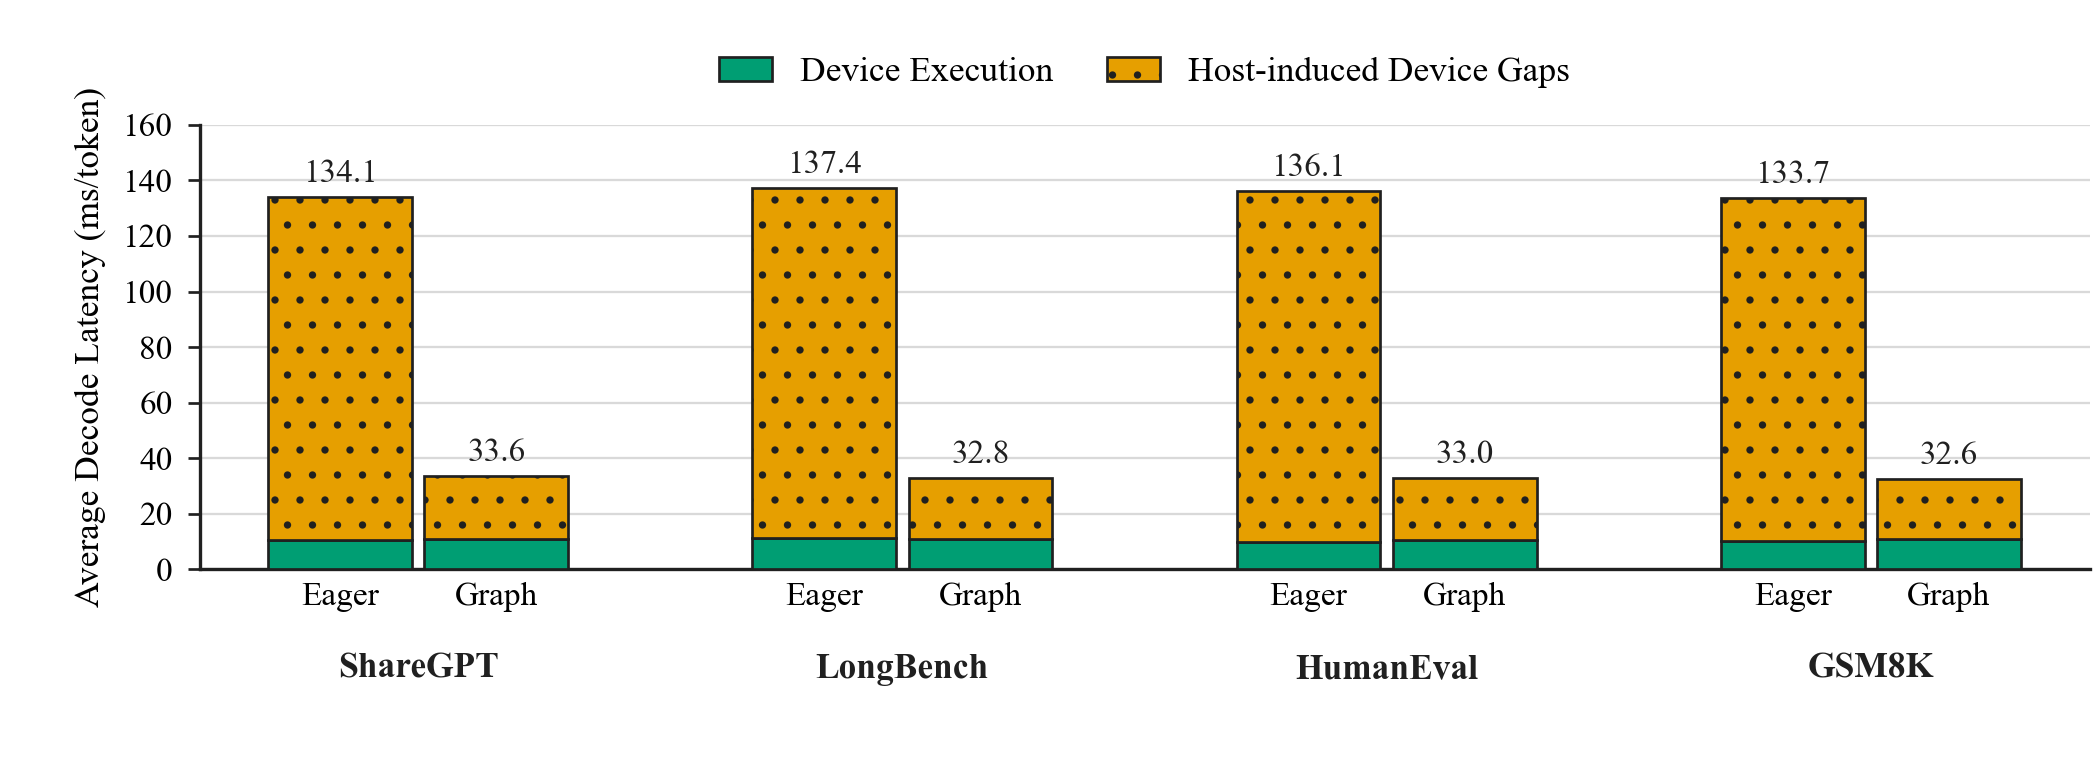
\includegraphics[width=1\linewidth]{figures/graph_breakdown.png} 
  \caption{Average decode latency breakdown under eager execution and graph replay. Graph replay substantially reduces host-induced device gaps while leaving device execution time nearly unchanged.} 
  \label{fig:graph_breakdown} 
\end{figure} 

However, graph replay is effective only when the captured execution state, including its memory bindings, remains stable. 
Dynamic expert offloading can violate this condition. 
A cache miss may trigger expert eviction and replacement, causing the logical-to-physical weight binding to change across decoding steps.
The captured computation then cannot safely reuse its previous bindings without repairing the graph or falling back to eager execution. 
Both options add host work and reduce the benefit of graph replay. 
The resulting systems problem is to \textbf{enable dynamic expert residency and placement without sacrificing graph replay under a bounded HBM budget }.

Graph-compatible inference runtimes take a different approach: they keep graph-visible workspaces, metadata, and execution configurations reusable across replays~\cite{ye2025flashinfer}. However, they do not support a bounded expert pool whose contents change dynamically. Therefore, existing systems lack an execution abstraction that supports dynamic expert replacement while preserving graph replay.

Our key insight is that \textbf{graph replay requires stable physical storage, not static expert residency}. Captured computation only requires its graph-visible storage addresses to remain valid. The runtime can therefore reuse a fixed set of physical slots for different logical experts: replacement changes slot contents and mapping values, not the addresses visible to the graph. This separation allows expert residency to evolve under a bounded HBM budget without invalidating replay.

Realizing this abstraction raises three systems challenges.
First, routing-dependent expert staging must occur without invalidating captured computation.
Active experts are known only after routing, yet loading and replacement must not alter the replay-visible storage or execution structure.
Second, bounded slot storage must be updated without placing expert transfer entirely on the critical path.
Changing routing decisions may require repeated expert movement, and the routed working set may exceed the available slots, making transfer--computation overlap essential for efficient execution.
Third, slot reuse must remain correct under asynchronous transfer and computation.
A slot cannot be reassigned while its previous contents are still in use, nor can a new assignment become visible before the staged weights are ready.

We present \system, a graph-compatible MoE offloading system that virtualizes dynamic logical experts over a fixed physical slot interface.
To isolate routing-dependent dynamism from captured computation, \system places expert staging at an eager boundary while keeping the physical storage seen by replayed kernels stable.
It further pipelines expert staging and computation through wave-based execution, allowing bounded slot storage to be reused while overlapping transfers for upcoming experts with ongoing computation.
Finally, a version-controlled handoff protocol coordinates transfer readiness,computation, and mapping publication to ensure safe slot reuse.
Together, these mechanisms preserve replay-stable execution while allowing expert residency and placement to evolve dynamically under constrained HBM.

In summary, this paper makes the following contributions:

\begin{itemize}

\item We identify a cross-layer conflict between dynamic expert offloading and graph replay in memory-constrained MoE inference: routing-driven expert replacement changes logical-to-physical weight bindings, whereas graph replay depends on a stable graph-visible execution state. 
From this conflict, we derive the key insight that replayability requires stable physical storage rather than static expert residency.

\item We design \system, a graph-compatible MoE offloading runtime that virtualizes dynamic logical experts over replay-stable physical slots.
\system isolates routing-dependent expert staging from captured computation, pipelines expert transfer with computation through wave-based execution, and coordinates safe slot reuse through a version-controlled handoff protocol.

\item We implement \system on top of vLLM-Ascend and evaluate it under constrained HBM. 
On Qwen3-30B-A3B, \system preserves exact model outputs and graph replay under dynamic expert offloading. Compared with graph-compatible full-layer staging, its multi-wave prefill execution reduces repeat-median TTFT p50 by 35.21\%.

\end{itemize}


\section{Background and Problem}
\label{sec:background}

\subsection{MoE residency under limited memory}

An MoE layer contains $E$ experts but routes each token to only $k \ll E$ of
them.  Sparse activation reduces compute, as in Switch Transformers
\cite{switch}, but not the capacity needed to make every expert available.
Offloading exploits temporal sparsity: inactive weights remain in host memory,
and the runtime caches or prefetches experts into a bounded device-resident
set.  Systems such as MoE-Infinity use activation traces to improve these
decisions \cite{moeinfinity}; FlexGen demonstrates the broader value of
coordinating model storage across heterogeneous memory \cite{flexgen}.

The runtime cost is determined not only by bytes transferred.  Demand loads can
stall a decode step, prefetches can contend with computation, and residency
updates can add host work.  For graph-based execution, residency also interacts
with capture validity.

\subsection{Why ordinary offloading breaks replay}

Graph replay records a repeated sequence of operations and their tensor
relationships.  A naive expert cache materializes the selected expert in a new
buffer or mutates the weight pointer used by the MoE kernel.  Both approaches
make the repeated decode iteration depend on dynamic host actions inside the
captured region.  Falling back to eager execution restores flexibility but
removes the optimization we seek to preserve.

We require four properties:

\begin{enumerate}
  \item \textbf{Address stability:} captured kernels reference a fixed set of
    device allocations.
  \item \textbf{Ownership safety:} a slot has one logical expert and cannot be
    overwritten while compute uses its current generation.
  \item \textbf{Capacity safety:} no route may silently exceed the configured
    slot budget.
  \item \textbf{Observable replay:} graph capture, replay, and fallback events
    are recorded and cannot be replaced by a forced eager success.
\end{enumerate}

\section{Design}
\label{sec:design}

\begin{figure}[t]
\centering
\fbox{\parbox{0.94\columnwidth}{
\centering
router output $\rightarrow$ placement plan $\rightarrow$ replay-boundary staging\\
$\downarrow$\\
pinned host experts $\rightarrow$ fixed device slot bank $\rightarrow$ captured MoE\\
$\uparrow$\hspace{5em}$\downarrow$\\
transfer events \hspace{4em} logical-to-physical mapping
}}
\caption{\system keeps tensor addresses stable and moves dynamic routing into
metadata and transfers outside the captured region.}
\label{fig:architecture}
\end{figure}

\subsection{Fixed-slot expert virtualization}

At initialization, \system allocates a fixed number of equal-shaped expert
slots.  A slot has a stable tensor address, an owner $(\ell,e)$ consisting of
layer and expert identifiers, and a monotonically increasing generation.
The logical-to-physical map translates a routed expert to its current slot.
Captured grouped matrix multiplications consume slot tensors and indices, not
fresh expert allocations.

The slot count is derived from the offload target, physical HBM, a KV-cache
reserve, and a minimum net-saving constraint.  Explicit capacity checks reject
an active working set that cannot be represented by the current execution
mode.  This prevents an apparently successful run from borrowing unaccounted
memory.

\subsection{Replay-boundary staging}

The router produces active expert identities.  A placement-plan adapter
computes retain, evict, demand-load, and optional prefetch sets.  The adapter is
deliberately policy-neutral: LRU or predictive control can be supplied by a
separate controller without changing the slot bank.

Staging occurs before the captured MoE region.  Host weights are copied on a
dedicated transfer stream, and the mapping is published only after the
corresponding load completes.  The graph then replays against stable slots.
No transfer or allocation is hidden inside the captured kernel sequence.

\subsection{Compute-protected lifecycle}

Each slot progresses through an ownership protocol: free, loading, ready,
computing, and eviction-pending.  Loading establishes a new owner and
generation.  Compute records the generation it consumes and protects that slot
until its completion event.  Eviction waits for both transfer and compute
dependencies.  Shutdown drains pending work before releasing storage.

The central safety invariant is:

\begin{quote}
A mapping may expose expert $(\ell,e)$ at slot $s$ only if $s$ is ready, owns
$(\ell,e)$, and its published generation equals the generation checked by the
consumer.
\end{quote}

Violations fail closed rather than selecting an eager path.

\subsection{Capacity-bounded wave prefill}

Prefill can route many tokens and activate more experts than the slot bank can
hold simultaneously.  \system partitions routed work into waves whose expert
set fits the bank.  For each wave, it stages missing experts, computes the
corresponding token subset, and restores output order before combining results.
With multiple staging buffers, the next wave's transfers can overlap the
current wave's compute.

Wave construction preserves token-to-expert assignments; it changes execution
order, not routing semantics.  Correctness tests compare the scattered and
restored output against the unpartitioned result.

\section{Implementation}
\label{sec:implementation}

\system is a Python package registered through vLLM's platform-plugin entry
point.  The implementation contains the slot bank, pinned host store, transfer
engine, prefill wave scheduler, automatic capacity configuration, profile
events, and fused-MoE adapters.  A hook-enabled vLLM-Ascend fork exposes the
boundaries at which routing, staging, and graph state can be coordinated.

The integration leaves request scheduling and the OpenAI-compatible API
unchanged.  Disabling the plugin restores the runtime's null hooks.  Native
weight-offload flags cannot be combined with \system because two independent
owners of expert storage would violate the slot invariant.

\section{Evaluation}
\label{sec:evaluation}

We separate implementation evidence from the experiments required to support a
submission claim.

\subsection{Current evidence}

The repository includes host-side tests for slot ownership, phase splitting,
wave restoration, graph guards, and benchmark artifact collection.  It also
includes the Issue~7 raw graph-only bundle for Qwen3-30B-A3B BF16 on one
Ascend 910B2, TP1, and 	exttt{max\_num\_seqs=1}.  Three independent service
starts each completed 11/11 ShareGPT requests and 1,408 output tokens; all
request token arrays matched exactly.  The bundle records stable slot
addresses for all 12 managed layers, generation and H2D ordering, bounded
multi-wave execution, replay issue timing, physical HBM samples, and release
acknowledgements.  Median TTFT across the starts was 537.70--573.64~ms and
median TPOT was 53.56--55.93~ms/token.  These values qualify the narrow runtime
path; they are not a matched performance comparison.

Historical capture-disabled diagnostics remain excluded because they lack the
raw, repeated contract and violate the graph-only evaluation boundary.

\subsection{Submission experiment matrix}

The checked-in harness defines real ShareGPT prompt buckets, graph-only cases,
14- and 28-GiB budgets, and artifact-preserving failure outcomes.
The final evaluation must answer four questions:

\begin{description}
  \item[Q1: Feasibility.] Does full residency fail under the same HBM/KV
    reservation for which \system serves requests successfully?
  \item[Q2: Graph compatibility.] Do capture and replay complete, and what
    fraction of decode steps replay without fallback?
  \item[Q3: Performance.] How do TTFT, TPOT, inter-token latency, throughput,
    and failure rate compare with matched graph-compatible native and legacy
    offload baselines?
  \item[Q4: Attribution.] What do fixed slots, asynchronous loading, transfer
    ordering, wave prefill, and automatic capacity selection each contribute?
\end{description}

Each cell requires three independent service starts and must report median and
dispersion.  Results must carry parent/runtime revisions, device identity,
model and workload digests, graph mode, HBM accounting, raw client metrics,
server logs, and transfer profiles.  Formal runs may use only an explicitly
reserved and idle physical NPU5 or NPU6.  A graph failure is retained as a
failed artifact and is not rerun with forced eager execution.

\section{Discussion and Limitations}

\paragraph{Policy is intentionally separate.}
\system supplies the data plane and a generic plan interface.  Predictive
placement, route-transition models, and EPLB comparisons belong to a separate
control-plane study.  This boundary allows all policies to share identical
slots, transfers, and graph behavior.

\paragraph{Current scope.}
The validated configuration is a single low-concurrency device and one
unquantized MoE model.  Multi-device expert parallelism changes the comparison
because its transfers are device-to-device rather than host-to-device.  Higher
concurrency can also change active-set size and overlap opportunities.

\paragraph{Evidence gap.}
The checked-in Issue~7 bundle closes the narrow graph replay and lifecycle
gate.  The remaining submission blocker is breadth: matched graph-compatible
baselines plus model, capacity, workload, and concurrency sensitivity.  Until
that matrix is complete, the paper supports a mechanism and narrow correctness
claim, not a general performance claim.

\section{Related Work}

MoE architectures use sparse routing to increase parameter capacity without
activating every parameter per token \cite{switch}.  DeepSpeed-MoE combines
model and parallelism techniques for large-scale MoE inference
\cite{deepspeedmoe}.  MoE-Infinity focuses on activation-aware caching and
prefetch for expert offloading \cite{moeinfinity}.  \system addresses a
different constraint: keeping the offload data plane compatible with captured
decode execution through stable slot addresses and an explicit lifecycle.

Heterogeneous inference systems such as FlexGen coordinate storage and
execution across device, host, and disk memory \cite{flexgen}.  vLLM uses
paged KV-cache management and continuous batching to improve LLM serving
\cite{vllm}.  \system is complementary: it virtualizes expert weights rather
than KV blocks and preserves the repeated MoE execution graph while residency
changes.

\section{Conclusion}

\system decouples dynamic expert identity from the stable addresses required
by graph replay.  Fixed slots, replay-boundary staging, protected ownership,
and wave prefill form a graph-compatible offload data plane.  The checked-in
Issue~7 artifact establishes its graph replay and lifecycle behavior across
three independent starts; matched, broader online evaluation remains necessary
to establish the breadth and magnitude of any performance benefit.

\bibliographystyle{plain}
\bibliography{references}

\end{document}
